\documentclass[11pt]{article}
\usepackage[left=1in, right=1in, top=1in, bottom=1in, includefoot]{geometry}		% Set margins to 1 inch.

% Reduce the vertical space above the title.
\usepackage{titling}
\setlength{\droptitle}{-8ex}

\usepackage{amsmath}				% For \text{}

\usepackage{amsthm}				% For proof environment
\usepackage{cleveref}
\newtheorem{lemma}{Lemma}
\newtheorem{theorem}{Theorem}

\usepackage{amsfonts}				% For \mathbb{}

\usepackage{graphicx}
\usepackage{floatrow}

\usepackage{nccmath}				% For fleqn environment

\usepackage{color}

\usepackage{bm}					% For \bm{}
\usepackage{physics}				% For \norm{}

\usepackage{enumerate}				% For customizing the numbering in the enumerate environment
%\usepackage{fitch}					% For Fitch-style proofs

\usepackage{tabularx}				% For making tables fit within page width
\usepackage{titlesec}				% For making the text of a section start on the same line as the section's title
\usepackage{url}					% For \url{}
\usepackage{hyperref}				% For breaking URLs
\def\UrlBreaks{\do\/\do-}				% For breaking URLs at '/' and '-'
\usepackage[T1]{fontenc}				% For fixing underscores in \url{}
\usepackage[labelformat=simple]{subcaption}				% For the subfigure environment
\renewcommand\thesubfigure{(\alph{subfigure})}		% For adding parentheses around subfigure references (Figure 2(a) instead of Figure 2a)

\newcommand{\colvect}[2]{
	\ensuremath{\big[\begin{smallmatrix}#1\\#2\end{smallmatrix}\big]}
}

% The \vspace command inside the \title command is used to reduce
% the space between the title and the author lines.
\title{Explaining Predictions of Deep Neural Networks \\ on the Yelp Dataset \\ Deliverable I}
\author{
	Caleb Kaiji Lu \\
	{\tt caleb.lu@andrew.cmu.edu}
	\and
	Selva Samuel \\
	{\tt ssamuel@andrew.cmu.edu}
}
\date{}

\begin{document}

\maketitle

\section{Progress Summary}

In our proposal, we stated that for deliverable I, we would train a state-of-the-art model for sentiment/rating prediction and explain predictions from the model using some functional methods. We were able to accomplish these goals for the most part.

\section{Implementation}

\subsection{Model Architecture}

In sentiment analysis tasks, most state-of-the-art methods use a combination of convolutional and recurrent neural networks. Convolutional neural networks, despite their use mainly in image-based applications, are also used in text-based applications which involve summarization of text since convolution can learn a holistic representation of a group of words instead of just individual words. Recurrent neural networks usually use the long short-term memory (LSTM) architecture to avoid the exploding gradient problem.

For our implementation, although our end goal is not to train a classifier that beats the best method for this dataset, we still want our model be as close to the best method as possible. The best accuracy so far for this data set has been 96\% \cite{Tang2015}. We were able to train a model whose validation accuracy is 93\%. 

The architecture that we used is shown in figure \ref{fig:dnn-arch}. The whole process takes about 20 minutes to train on 200,000 reviews. We trained our neural network on a server with a 64-bit Intel Xeon processor and 128GB RAM. The details of the model will not be discussed in this report.

We used the Keras\footnote{\url{https://keras.io}} deep learning framework for implementing our neural network. Keras is a high-level deep learning framework. It can use Theano\footnote{\url{http://deeplearning.net/software/theano/}} or TensorFlow\footnote{\url{https://www.tensorflow.org}} as its backend. We ran Keras on top of TensorFlow.

\begin{figure}
	\includegraphics[width=\textwidth]{figure1}
	\caption{Architecture of deep neural network used for sentiment analysis in the Yelp dataset}
	\label{fig:dnn-arch}
\end{figure}

\subsection{Explanation Generation}

We used two methods to explain the predictions from our trained neural network - integrated gradients and masking. We explain both of these approaches in the following subsections.

\subsubsection{Integrated Gradients}

In order to generate explanations using integrated gradients, we adapted the method introduced by Ribeiro et al. \cite{Ribeiro2016}. In neural networks, gradients on the input data can be used as an indication explanation. Integrated gradients provide a better way for explanation using gradients. They can be calculated by using the following formula:

\[
	\mathsf{IntegratedGrads}_i(x) ::= (x_i - x_i') \times \int_0^1 \frac{\partial F(x' + \alpha \times (x - x'))}{\partial x_i} d\alpha
\]

As demonstrated in \cite{Ribeiro2016}, the integrated gradient metric performs well on some image and language tasks.

We applied the integrated gradients method to our model and got sound results overall. In figure \ref{fig:int-grad:pos}, for example, word ``the'' and ``is'' are assigned relatively fewer weights while the words ``food'' and ``amazing'', which are words more central to the sentiment of this sentence, are assigned more weight. Similarly in figure \ref{fig:int-grad:neg}, words such as ``really'', ``hate'' and ``tastes'' are assigned more weight than the other words.

\begin{figure}[H]
	\centering
	\begin{subfigure}{0.45\textwidth}
		\centering
		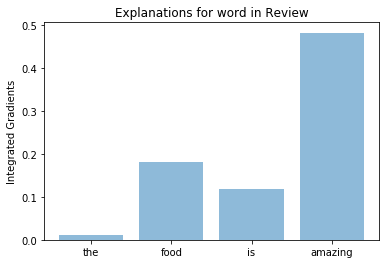
\includegraphics[width=\linewidth]{figure2}
		\caption{Positive review}
		\label{fig:int-grad:pos}
	\end{subfigure} % There should be no newlines here.
	\begin{subfigure}{0.45\textwidth}
		\centering
		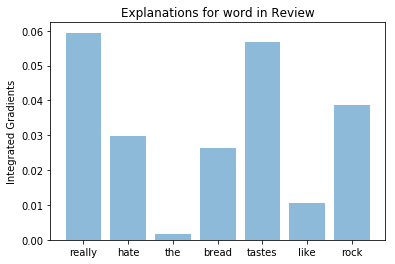
\includegraphics[width=\linewidth]{figure3}
		\caption{Negative review}
		\label{fig:int-grad:neg}
	\end{subfigure}
	\caption{Explanations generated by using integrated gradients}
\end{figure}

However, this method is not robust for longer reviews. When a review is longer than a few words, it tends to allocate more weight on words occurring in the first half of the review text. The reason behind this is not well-understood now, but we will investigate more by tuning the integrated gradients framework.

\subsubsection{1-gram Masking}

The second method that we used to generate explanations of predictions made by our trained neural network is 1-gram masking. In natural language processing, an n-gram refers to a contiguous sequence of n words in a piece of text. So, 1-gram is just a single word. In 1-gram masking, the importance of a word in making a correct prediction is determined by the magnitude of the change in the prediction score when all occurrences of the word are removed from the text. The larger the change in the prediction score, the greater is its influence on making the correct prediction. Figure \ref{fig:mask} shows the explanations generated by using 1-gram masking on a negative and a positive review in our dataset.

\begin{figure}
	\centering
	\begin{subfigure}{0.45\textwidth}
		\centering
		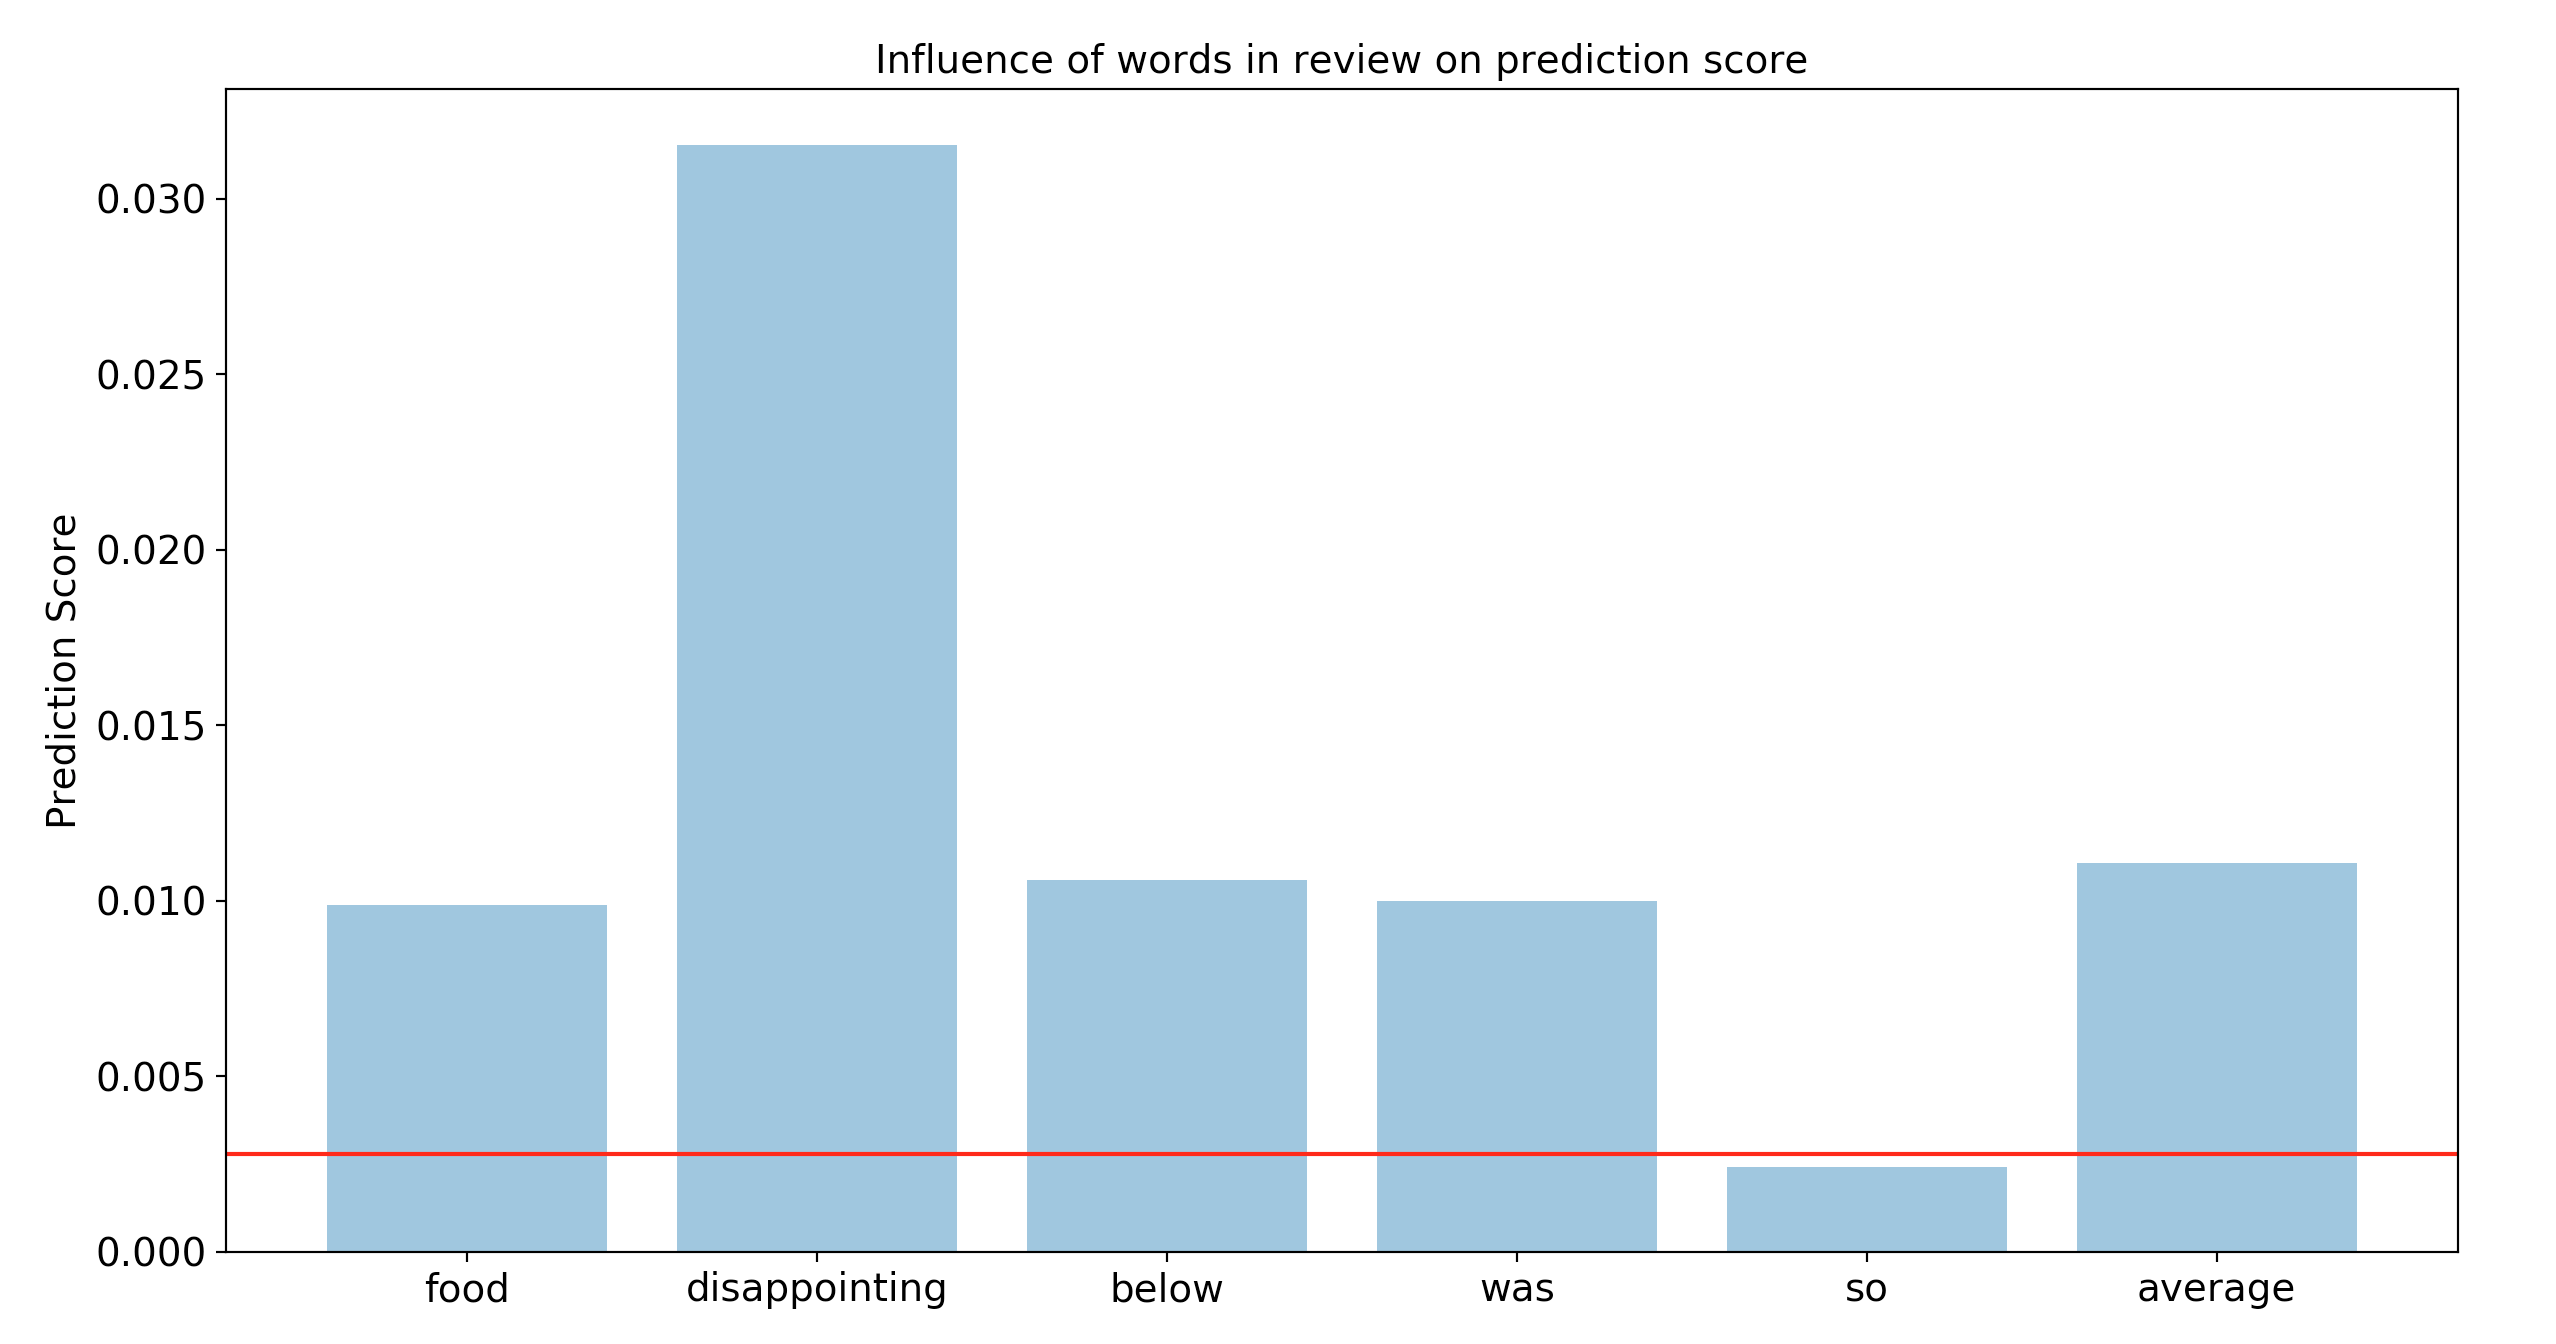
\includegraphics[width=\linewidth]{figure5}
		\caption{Negative review}
		\label{fig:mask:neg}
	\end{subfigure} % There should be no newlines here.
	\begin{subfigure}{0.45\textwidth}
		\centering
		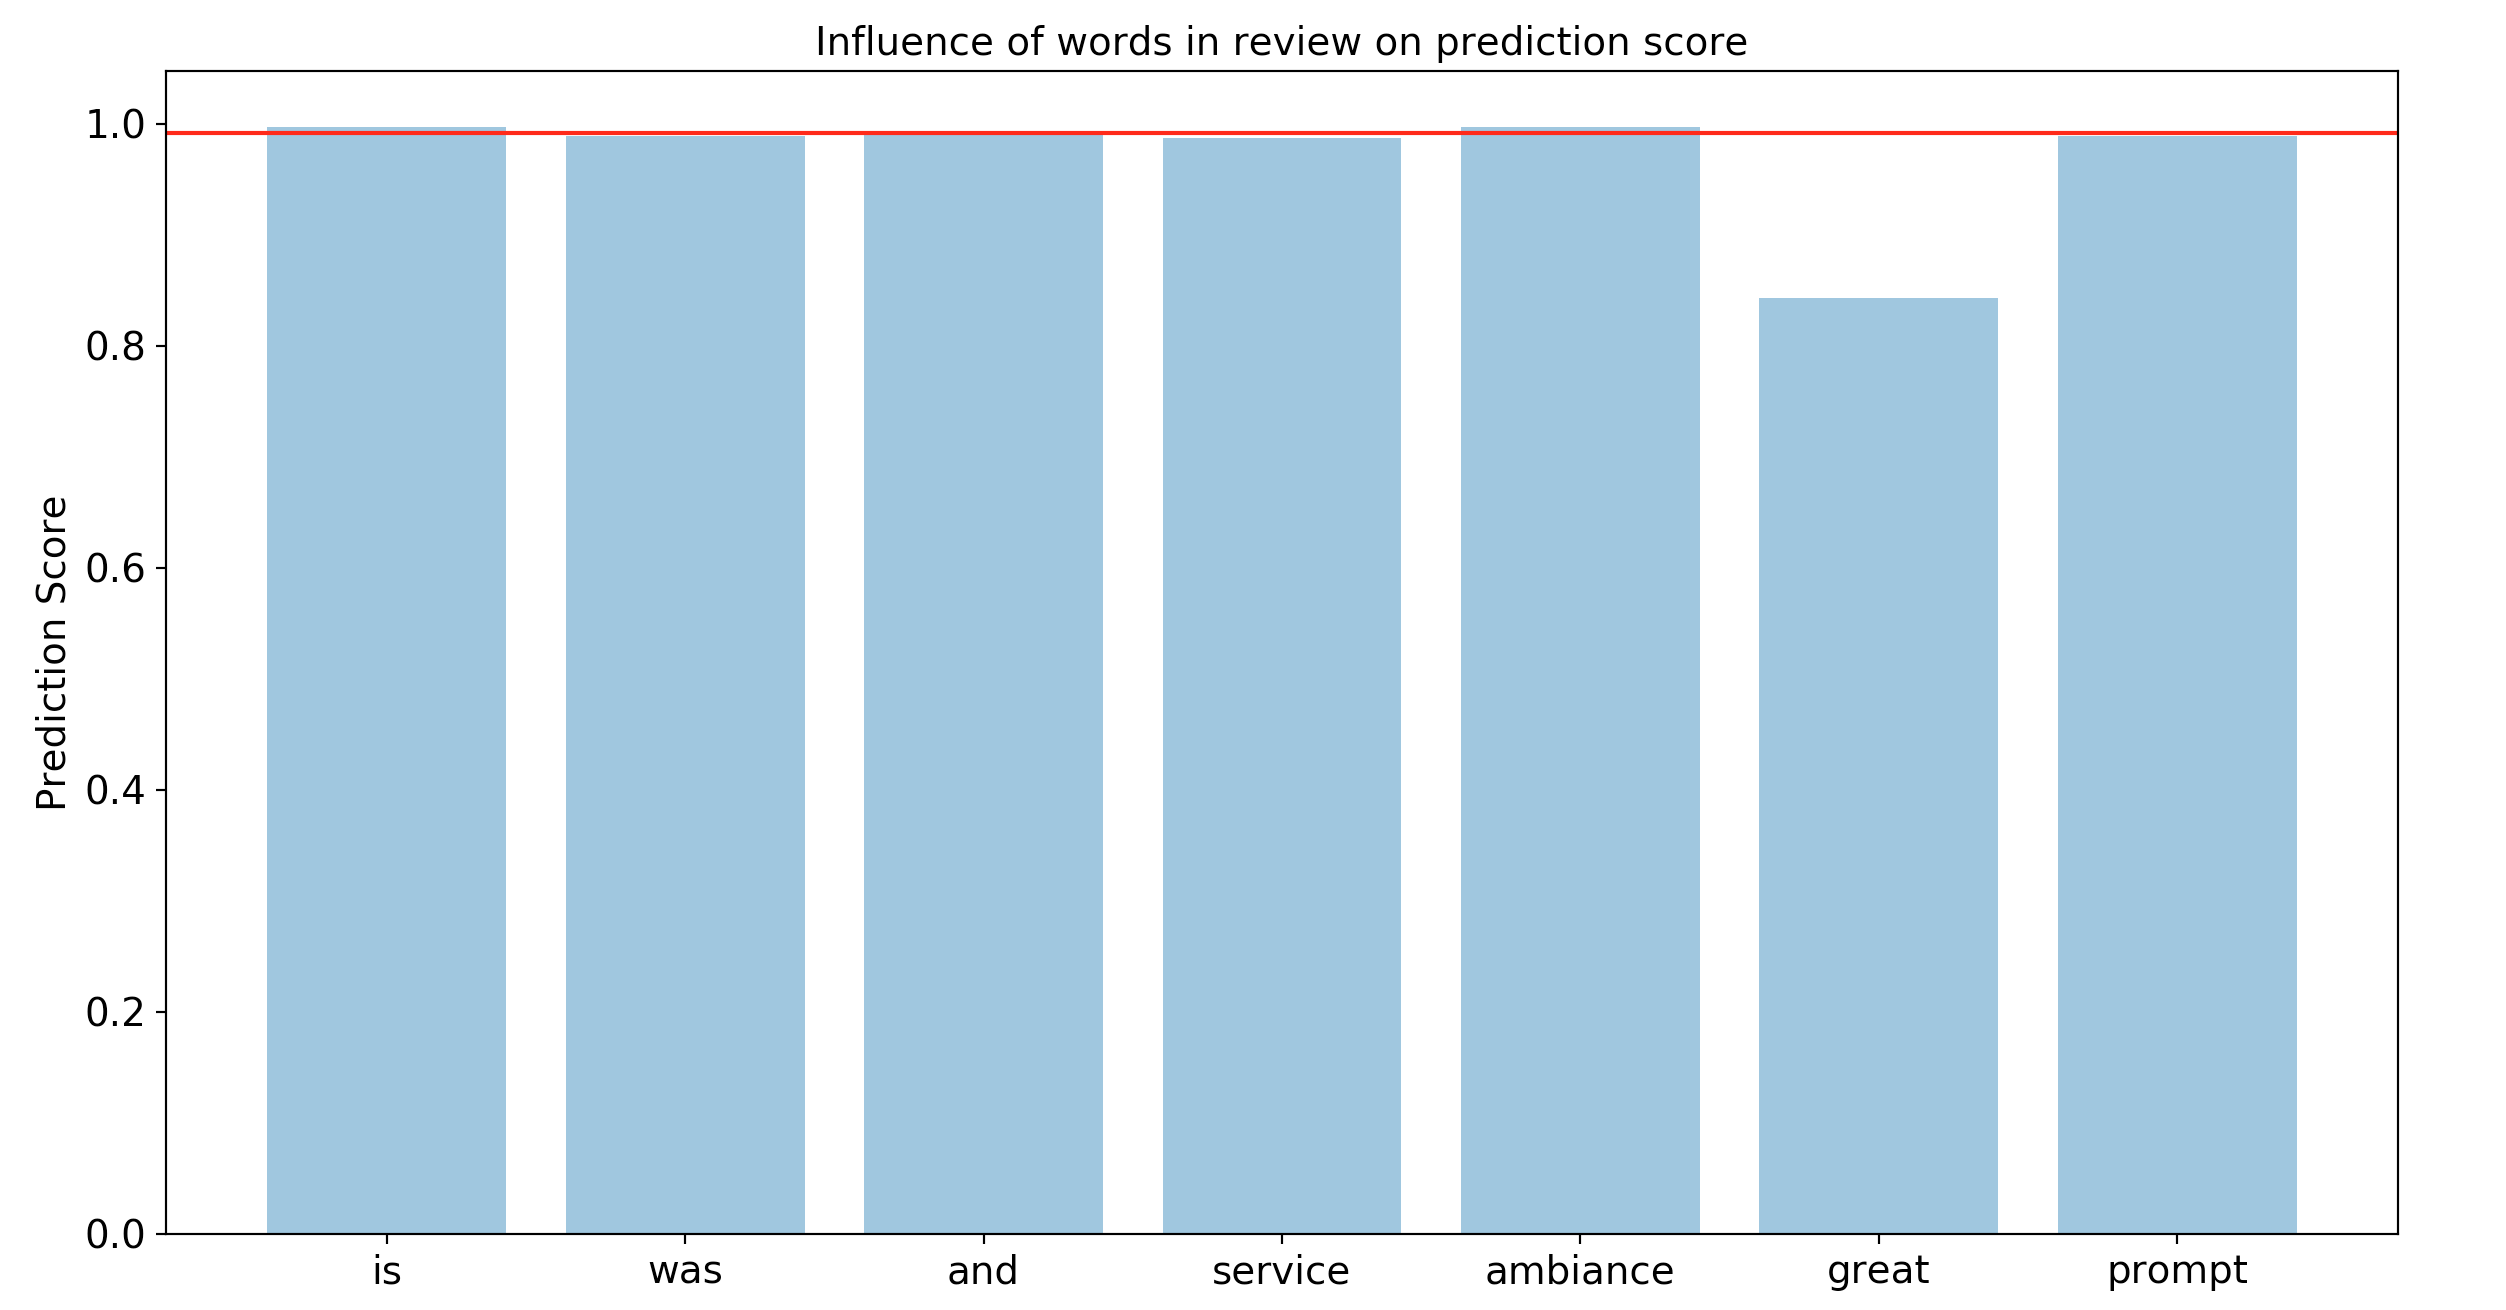
\includegraphics[width=\linewidth]{figure4}
		\caption{Positive review}
		\label{fig:mask:pos}
	\end{subfigure}
	\caption{Explanations generated by using 1-gram masking}
	\label{fig:mask}
\end{figure}

\section{Future Work}

\subsection{Improving the explanation models}

As mentioned above, we will be improving the integrated gradients method so that it can generate better explanations.

\subsection{Implementing QII}

This week, we are going to implement the QII method \cite{Datta2017} for our model since the explanations generated by QII can help us understand questions like ``What are some important words for a positive review for a Mexican restaurant?'' using a quantity of interest for a group of features. One challenge for implementing QII for text data, especially for a task like sentiment analysis, is that the feature space is large, and it is hard to define ``the intervention'' for a specific word.

\subsection{Implementing gender prediction}

Starting next week, we are going to implement gender prediction and see if gender of the user behind each review can be accurately predicted by the review text alone. If so, we would analyze the privacy implication and repair the model using some privacy theories mentioned in class.

\bibliographystyle{abbrv}
\bibliography{references}

\end{document}
